\documentclass[12pt]{article}
\usepackage{fontspec}
\usepackage{xeCJK}
\setCJKmainfont[AutoFakeBold=2]{SimSun}
%\setCJKsansfont{SimHei}
\usepackage{amsmath, amssymb, amsthm}
\usepackage{geometry}
\usepackage{tikz}
\usepackage{fancyhdr}
%\setlength{\headheight}{15pt}
\usetikzlibrary{calc, intersections} % ABX 用於某些符號，若無可刪除
\usepackage{enumitem}
\usepackage{tkz-euclide}
\usepackage{subcaption}
\usepackage{indentfirst}
\usepackage{float}
\usepackage{chngcntr}
\counterwithin{figure}{section}
\counterwithin{figure}{subsection}
\usepackage[most]{tcolorbox}
\usepackage{etoolbox}
% 1. 定義一個新的開關，名字可以自訂（例如：showanswer）
\newtoggle{showanswer}

% 2. 設置開關狀態：true 為開啟（編譯），false 為關閉（不編譯）
\settoggle{showanswer}{true}

\newtcolorbox{mybox}[4][證明]{
  empty,
  breakable,                % 支援跨頁
  sharp corners,
  left=#2+#3,               % 為左側標籤預留空間 (縮進)
  right=0pt, top=0pt, bottom=0pt,
  colback=white,
  % --- 加入以下這行來調整段距 ---
  before upper={\setlength{\parskip}{0.5em plus 0.2em minus 0.1em}},
  after={\vspace{#4}},
  % ---------------------------
  overlay unbroken and first={ % 在第一頁/未斷頁時繪製標籤
    \node[
      anchor=north west,
      draw, 
      inner sep=0pt,
      minimum width=#2,
      minimum height=1.6em, 
      font=\bfseries\boldmath
    ] at (frame.north west) {#1};
  }
}

\geometry{left=1.5cm, right=1.5cm, top=2cm, bottom=2cm}
\counterwithout{figure}{subsection}
% 設定頁首頁尾
\pagestyle{fancy}
\fancyhf{}
\renewcommand{\headrulewidth}{2pt}
\renewcommand{\thefigure}{\thesection-\arabic{figure}} % 主圖編號
\renewcommand{\thesubfigure}{圖 \thesection-\arabic{figure}} % 子圖變為 2-1
\captionsetup[figure]{labelformat=simple, labelsep=quad} 
\captionsetup[subfigure]{labelformat=simple, labelsep=quad} % 移除括號
\renewcommand{\figurename}{圖}
\lhead{廖汶鋒}
\chead{幾何練習題}
\rhead{澳門培道中學}
\fancyfoot[C]{\thepage} % Centered footer
%\fancyfoot[L]{2026年2月7日} % Left footer

%\title{四點共圓}
%\author{廖汶鋒}
%\date{2026年2月7日}
\linespread{1.3}

% 定段落首行縮進（兩個中文字）
\setlength{\parindent}{2em}
\setlength{\headheight}{15pt} % 避免頁首高度警告
\begin{document}
\thispagestyle{fancy}  % 讓首頁也顯示頁首
%\maketitle
\begin{center}
    \textbf{\Large{幾何練習題}}
\end{center}

\begin{mybox}[習題 1]{5em}{1em}{0.5em}
    $\odot{O_1}$和$\odot{O_2}$相交點$X$和$Y$。直線$l_1$通過$O_1$且與$\odot{O_2}$相交於點$P$和$Q$；
    直線$l_2$通過$O_2$且與$\odot{O_1}$相交於點$R$和$S$。若$P$、$Q$、$R$、$S$四點共圓且圓心為$O$，
    
    求證：$O$、$X$、$Y$三點共線。
\end{mybox}
\begin{mybox}[畫法 1-1]{5em}{1em}{0.5em}
    千萬不能傻更更地按順序畫圖，否則你就會被困在「$P$、$Q$、$R$、$S$四點共圓」的陷阱中。

    幾何題作圖必須要懂得一個原則：
    \begin{quotation}
        \centering
        盡可能把「如果」刪除，重新敍述題目。
    \end{quotation}

    我們利用作圖法來重新敍述這條題目：

    第一步，畫出$\odot{O_1}$和$O_2$，一般$O_2$可以選在$\odot{O_1}$外；畫出任一通過$O_2$的直線$l_2$，與$\odot{O_1}$相交於點$R$和$S$；
    \begin{figure}[H]
        \centering
        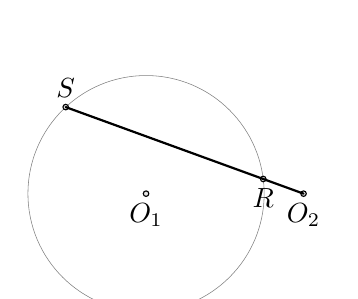
\begin{tikzpicture}[scale=0.5]
            \tkzDefPoints{-2/0/O_1, 2/0/O_2, 1/0/A}
            \tkzDefPointBy[rotation=center O_2 angle -20](O_1) \tkzGetPoint{Z}
            \tkzInterLC(O_2,Z)(O_1,A) \tkzGetPoints{R}{S}
            %\tkzDefLine[mediator](R,S) \tkzGetPoints{m_S}{m_R}
            %\tkzDefPointWith[linear, K=0.9](m_S,m_R) \tkzGetPoint{O}
            %\tkzDefPointBy[projection=onto O--O_2](O_1) \tkzGetPoint{D_1}
            %\tkzInterLC(O_1,D_1)(O,R) \tkzGetPoints{P}{Q}
            %\tkzInterCC(O_1,R)(O_2,P) \tkzGetPoints{X}{Y}
            \tkzDrawCircle(O_1,R)
            %\tkzDrawCircle(O,R)
            \tkzDrawPoints(O_1,O_2,R,S)
            \tkzLabelPoints[below](O_1,O_2,R)
            \tkzLabelPoints[above](S)
            \tkzDrawSegments[black, thick](O_2,S)
            %\tkzDrawSegments[black, thick, dashed](O,O_1)
            %\tkzLabelPoints[right](X)
            %\tkzMarkRightAngle[color=red](O,D_1,O_1)
        \end{tikzpicture}
    \end{figure}

    第二步，畫出線段$RS$的中垂線$m_{RS}$，並在其上任取一點記為$O$；以$O$點為圓心，$OR$為半徑畫圓，此圓記為$\odot{O}$。
    \begin{figure}[H]
        \centering
        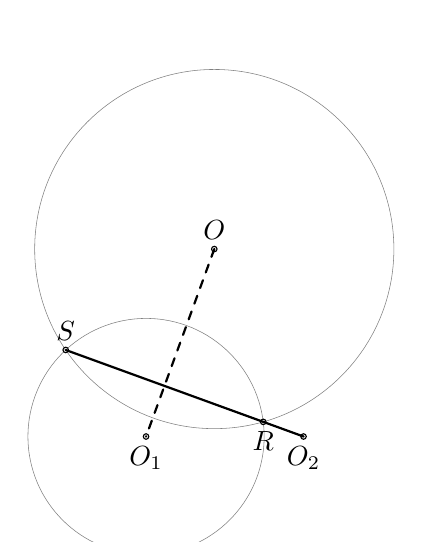
\begin{tikzpicture}[scale=0.5]
            \tkzDefPoints{-2/0/O_1, 2/0/O_2, 1/0/A}
            \tkzDefPointBy[rotation=center O_2 angle -20](O_1) \tkzGetPoint{Z}
            \tkzInterLC(O_2,Z)(O_1,A) \tkzGetPoints{R}{S}
            \tkzDefLine[mediator](R,S) \tkzGetPoints{m_S}{m_R}
            \tkzDefPointWith[linear, K=0.9](m_S,m_R) \tkzGetPoint{O}
            %\tkzDefPointBy[projection=onto O--O_2](O_1) \tkzGetPoint{D_1}
            %\tkzInterLC(O_1,D_1)(O,R) \tkzGetPoints{P}{Q}
            %\tkzInterCC(O_1,R)(O_2,P) \tkzGetPoints{X}{Y}
            \tkzDrawCircle(O_1,R)
            \tkzDrawCircle(O,R)
            \tkzDrawPoints(O_1,O_2,R,S,O)
            \tkzLabelPoints[below](O_1,O_2,R)
            \tkzLabelPoints[above](S,O)
            \tkzDrawSegments[black, thick](O_2,S)
            \tkzDrawSegments[black, thick, dashed](O,O_1)
            %\tkzLabelPoints[right](X)
            %\tkzMarkRightAngle[color=red](O,D_1,O_1)
        \end{tikzpicture}
    \end{figure}

    如何確定$P$和$Q$點的位置，即如何找出通過$O_1$的直線$l_1$？這個答案不難導出，依題意可知$OP=OQ$及$O_2P=O_2Q$，所以$P$和$Q$關於$OO_2$軸對稱，可推導出$PQ\perp OO_2$，即$l_1\perp OO_2$。
    基於這個結論，我們可以繼續作圖：

    第三步，連結$OO_2$，過點$O_1$作直線$l_1\perp OO_2$，且與$\odot{O}$相交於點$P$和$Q$；
    \begin{figure}[H]
        \centering
        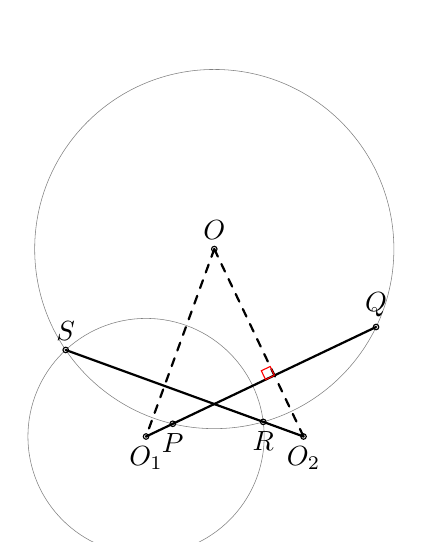
\begin{tikzpicture}[scale=0.5]
            \tkzDefPoints{-2/0/O_1, 2/0/O_2, 1/0/A}
            \tkzDefPointBy[rotation=center O_2 angle -20](O_1) \tkzGetPoint{Z}
            \tkzInterLC(O_2,Z)(O_1,A) \tkzGetPoints{R}{S}
            \tkzDefLine[mediator](R,S) \tkzGetPoints{m_S}{m_R}
            \tkzDefPointWith[linear, K=0.9](m_S,m_R) \tkzGetPoint{O}
            \tkzDefPointBy[projection=onto O--O_2](O_1) \tkzGetPoint{D_1}
            \tkzInterLC(O_1,D_1)(O,R) \tkzGetPoints{P}{Q}
            %\tkzInterCC(O_1,R)(O_2,P) \tkzGetPoints{X}{Y}
            \tkzDrawCircle(O_1,R)
            \tkzDrawCircle(O,R)
            \tkzDrawPoints(O_1,O_2,R,S,O,P,Q)
            \tkzLabelPoints[below](O_1,O_2,P,R)
            \tkzLabelPoints[above](Q,S,O)
            \tkzDrawSegments[black, thick](O_1,Q O_2,S)
            \tkzDrawSegments[black, thick, dashed](O,O_1 O,O_2)
            %\tkzLabelPoints[right](X)
            \tkzMarkRightAngle[color=red](O,D_1,O_1)
        \end{tikzpicture}
    \end{figure}

    此時，$\odot{O_2}$的半徑才可以被$OP$所確定。

    第四步，以$O_2$點為圓心，$OP$為半徑畫圓，此圓記為$\odot{O_2}$，並標出$\odot{O_2}$與$\odot{O_1}$的交點$X$和$Y$。
    \begin{figure}[H]
        \centering
        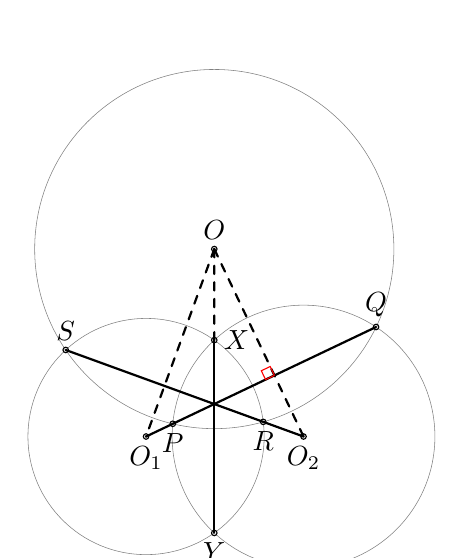
\begin{tikzpicture}[scale=0.5]
            \tkzDefPoints{-2/0/O_1, 2/0/O_2, 1/0/A}
            \tkzDefPointBy[rotation=center O_2 angle -20](O_1) \tkzGetPoint{Z}
            \tkzInterLC(O_2,Z)(O_1,A) \tkzGetPoints{R}{S}
            \tkzDefLine[mediator](R,S) \tkzGetPoints{m_S}{m_R}
            \tkzDefPointWith[linear, K=0.9](m_S,m_R) \tkzGetPoint{O}
            \tkzDefPointBy[projection=onto O--O_2](O_1) \tkzGetPoint{D_1}
            \tkzInterLC(O_1,D_1)(O,R) \tkzGetPoints{P}{Q}
            \tkzInterCC(O_1,R)(O_2,P) \tkzGetPoints{X}{Y}
            \tkzDrawCircle(O_1,R)
            \tkzDrawCircle(O_2,P)
            \tkzDrawCircle(O,R)
            \tkzDrawPoints(O_1,O_2,R,S,O,P,Q,X,Y)
            \tkzLabelPoints[below](O_1,O_2,Y,P,R)
            \tkzLabelPoints[above](Q,S,O)
            \tkzDrawSegments[black, thick](O_1,Q O_2,S X,Y)
            \tkzDrawSegments[black, thick, dashed](O,O_1 O,X O,O_2)
            \tkzLabelPoints[right](X)
            \tkzMarkRightAngle[color=red](O,D_1,O_1)
        \end{tikzpicture}
    \end{figure}

    這樣一來，本題的幾何圖才算是「重構」完成了。
\end{mybox}
\begin{mybox}[解答 1-1]{5em}{1em}{0.5em}
    由幾何圖明顯看到「三根軸交於一點」的事實，所以這道題顯然就是利用根心定理去完成的。

    設$PQ$交$RS$於點$T$。
    
    因為$PQ$是$\odot{O}$和$\odot{O_2}$的公共弦、$RS$是$\odot{O}$和$\odot{O_1}$的公共弦、$XY$是$\odot{O_1}$和$\odot{O_2}$的公共弦，
    由根心定理可知$PQ$、$RS$、$XY$交於同一點，即$X$、$Y$、$T$三點共線。

    利用根軸的性質可知$PQ\perp OO_2$及$RS\perp OO_1$，即有$O_1T\perp OO_2$及$O_2T\perp OO_1$，所以$T$是$\triangle{OO_1OO_2}$的垂心，
    因此有$OT\perp O_1O_2$。

    再次利用根軸的性質可知$XY\perp O_1O_2$，所以直線$OT$和$XY$互相平行或重合。最後結合$T$點在$XY$上可知，直線$OT$和$XY$重合，所以有$O$、$X$、$Y$、$T$四點共線。
\end{mybox}
\begin{mybox}[反思]{4em}{1em}{0.5em}
    「這個解答已經完備了嗎？」這個問題是你在每次解題後必須要問自己的關鍵問題。

    回顧上述的解答，一切都是基於「$PQ$與$RS$相交」為大前提才能去推導的，我們必須要思考「$PQ$與$RS$平行」這種情況是否會發生？如果會，那麼解答就不完備了。

    不妨設$PQRS$是凸四邊形。若$PQ$與$RS$平行，結合$P$、$Q$、$R$、$S$四點共圓可知，$PQRS$是一個「等腰梯形」或「矩形」。

    無論是「等腰梯形」還是「矩形」，它們都有一個共通點：一對平行邊共用同一條中垂線。換言之，$PQ$與$RS$平行的情況下，線段$PQ$和$RS$的中垂線會重合。

    因為$O_1$在$RS$的中垂線上，$O_2$在$PQ$的中垂線上，所以直線$O_1O_2$為線段$PQ$和$RS$的公共中垂線。

    又因為$O_1$、$P$、$Q$三點共線，結合「直線$O_1O_2$為線段$PQ$和$RS$的公共中垂線」，所以$O_1$為$PQ$的中點，同理可得$O_2$為$RS$的中點。

    此時，$\odot{O_1}$和$\odot{O_2}$的圓心和半徑都被唯一確定了，$\odot{O}$也被圓內接四邊形$PQRS$唯一確定了。
\end{mybox}
\begin{mybox}[畫法 1-2]{5em}{1em}{0.5em}
    按照「反思」的部分去畫出第二種情況的幾何圖：

    第一步，以任一點$O$和任意半徑畫出$\odot{O}$，畫出一對分別與$\odot{O}$相交的平行線$\left(l_3,l_4\right)$，記$l_3$交$\odot{O}$於點$P$和$Q$，記$l_4$交$\odot{O}$於點$R$和$S$。
    \begin{figure}[H]
        \centering
        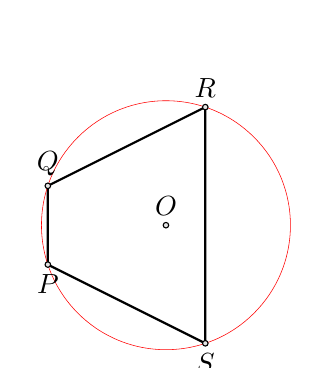
\begin{tikzpicture}[scale=0.5]
            \tkzDefPoints{-2/-1/P, -2/1/Q, -2/0/O_1, 2/3/R, 2/-3/S, 2/0/O_2}
            \tkzDefTriangleCenter[circum](P,Q,R) \tkzGetPoint{O}
            \tkzDrawPolygon[black, thick](P,Q,R,S)
            %\tkzDrawCircle(O_1,R)
            %\tkzDrawCircle(O_2,P)
            \tkzDrawCircle[red](O,P)
            %\tkzInterCC(O_1,R)(O_2,P) \tkzGetPoints{X}{Y}
            \tkzDrawPoints(P,Q,R,S,O)
            %\tkzDrawSegments[black, thick](O_1,O_2 X,Y)
            \tkzLabelPoints[below](P,S)
            \tkzLabelPoints[above](Q,R,O)
            %\tkzLabelPoints[left](O_1)
            %\tkzLabelPoints[right](O_2)
        \end{tikzpicture}
    \end{figure}

    第二步，畫出線段$RS$的中垂線$m_{RS}$，此直線必定通過$O$點。作$m_{RS}$分別交$PQ$、$RS$於$O_1$、$O_2$兩點。
    \begin{figure}[H]
        \centering
        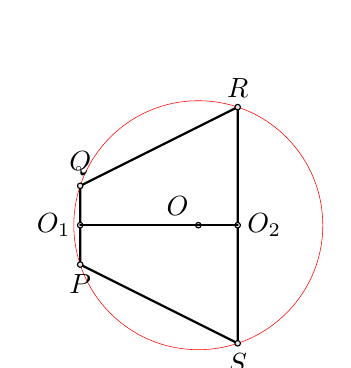
\begin{tikzpicture}[scale=0.5]
            \tkzDefPoints{-2/-1/P, -2/1/Q, -2/0/O_1, 2/3/R, 2/-3/S, 2/0/O_2}
            \tkzDefTriangleCenter[circum](P,Q,R) \tkzGetPoint{O}
            \tkzDrawPolygon[black, thick](P,Q,R,S)
            %\tkzDrawCircle(O_1,R)
            %\tkzDrawCircle(O_2,P)
            \tkzDrawCircle[red](O,P)
            %\tkzInterCC(O_1,R)(O_2,P) \tkzGetPoints{X}{Y}
            \tkzDrawPoints(P,Q,R,S,O_1,O_2,O)
            \tkzDrawSegments[black, thick](O_1,O_2)
            \tkzLabelPoints[below](P,S)
            \tkzLabelPoints[above](Q,R)
            \tkzLabelPoints[above left](O)
            \tkzLabelPoints[left](O_1)
            \tkzLabelPoints[right](O_2)
        \end{tikzpicture}
    \end{figure}

    第三步，以$O_1$點為圓心，$OR$為半徑畫圓，此圓記為$\odot{O_1}$；以$O_2$點為圓心，$OP$為半徑畫圓，此圓記為$\odot{O_2}$。最後畫出$\odot{O_1}$和$\odot{O_2}$的交點$X$和$Y$。
    \begin{figure}[H]
        \centering
        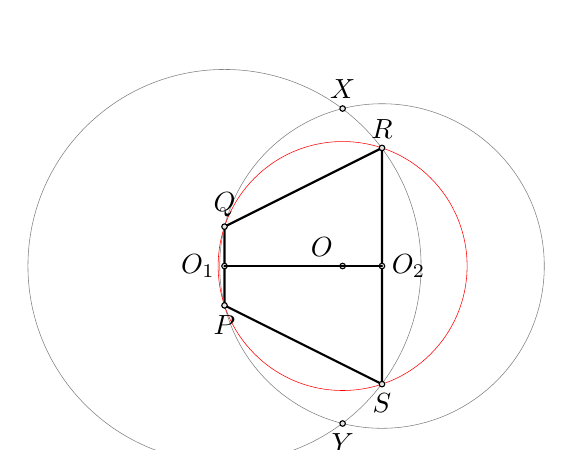
\begin{tikzpicture}[scale=0.5]
            \tkzDefPoints{-2/-1/P, -2/1/Q, -2/0/O_1, 2/3/R, 2/-3/S, 2/0/O_2}
            \tkzDefTriangleCenter[circum](P,Q,R) \tkzGetPoint{O}
            \tkzDrawPolygon[black, thick](P,Q,R,S)
            \tkzDrawCircle(O_1,R)
            \tkzDrawCircle(O_2,P)
            \tkzDrawCircle[red](O,P)
            \tkzInterCC(O_1,R)(O_2,P) \tkzGetPoints{X}{Y}
            \tkzDrawPoints(P,Q,R,S,O_1,O_2,O,X,Y)
            \tkzDrawSegments[black, thick](O_1,O_2)
            \tkzLabelPoints[below](P,Y,S)
            \tkzLabelPoints[above](Q,X,R)
            \tkzLabelPoints[above left](O)
            \tkzLabelPoints[left](O_1)
            \tkzLabelPoints[right](O_2)
        \end{tikzpicture}
    \end{figure}
\end{mybox}\begin{mybox}[解答 1-2]{5em}{1em}{0.5em}
    若$PQ$與$RS$平行，因為$PQ$是$\odot{O}$和$\odot{O_2}$的公共弦、$RS$是$\odot{O}$和$\odot{O_1}$的公共弦、$XY$是$\odot{O_1}$和$\odot{O_2}$的公共弦，
    由根心定理可知$PQ$、$RS$、$XY$互相平行且$O$、$O_1$、$O_2$三點共線。

    記$\odot{O}$、$\odot{O_1}$和$\odot{O_2}$的半徑分別為$r$、$r_1$和$r_2$。原命題等價於以下的命題一：
    \begin{equation*}
        \text{$O$在$\odot{O_1}$和$\odot{O_2}$的根軸上}\quad\Leftrightarrow\quad O_1O^2-r_1^2=O_2O^2-r_2^2
    \end{equation*}
    容易證明得
    \begin{align*}
        O_1O^2-r_1^2&=r^2-\left(\frac{1}{2}PQ\right)^2-\left[O_1O_2^2+\left(\frac{1}{2}RS\right)^2\right]\\
        &=r^2-\left(\frac{1}{2}RS\right)^2-\left[O_1O_2^2+\left(\frac{1}{2}PQ\right)^2\right]\\
        &=O_2O^2-r_2^2
    \end{align*}
    命題一成立，原命題得證。
\end{mybox}

\end{document}